\documentclass{scrartcl}
\usepackage{ngerman}
\usepackage{url}
\usepackage{graphicx}
\usepackage{float}
\usepackage{placeins}

\title{Masterprojekt: Ähnlichkeitssuche in Multimedia-Daten}
\subtitle{Projektbericht}
\author{Christian Brzeski \and Jean Pierre Bineyti}
\date{\today}

\begin{document}
\maketitle

\section{Aufgabenstellung}
Im Masterprojekt Informationssysteme haben wir uns mit der Ähnlichkeitssuche zwischen Multimediadaten beschäftigt. Der Fokus liegt dabei auf Fotos, welche auf Basis von sogenannten Signaturen ausgewertet und über verschiedene Distanzmaße miteinander verglichen werden sollen. Über die entsprechenden Distanzen sollen Ähnlichkeiten zwischen Bildern gemessen und  diese dann entsprechend kategorisiert und indexiert werden. Diese instanzbasierten Suche bildet eine Alternative zur Tag-basierten Ähnlichkeitssuche, bei welcher die Ähnlichkeit zwischen multimedialen Objekten auf Basis von Übereinstimmungen eben solcher Tags bemessen wird. Im weiteren Vorgehen haben wir uns speziell auf Fotos im jpg.- Format aus dem Internet fokussiert. Unser Ziel ist es dabei uns ein Bild der bestehenden Technologien im Bereich Computer Vision zu machen und unterschiedliche Ansätze bei der Ähnlichkeitssuche zu testen und zu vergleichen. Abgeschlossen wird das Projekt mit einem Prototypen, der von uns programmiert und dokumentiert wird. Dieser soll den Grundanforderungen der Ähnlichkeitssuche genügen und invariant gegenüber Rotation und Skalierung sowie kleinen Veränderungen im Bild sein.

\section{Implementierung}

\subsection{Vorbereitung}

Nachdem wir uns in unseren Teams eingefunden und untereinander ausgetauscht haben, haben wir mit der ersten Verteilung von Arbeitspaketen und mit der Einrichtung einer passenden Projektumgebung begonnen. Als Versionsverwaltung und Plattform für kollaboratives Arbeiten haben wir uns für Git entschieden und als Programmiersprache haben wir uns auf Java beschränkt, da es hierfür zahlreiche Frameworks im Bereich Computer Vision gibt und wir beide mit der Sprache gut vertraut sind. 
\\
\\
Zunächst haben wir drei verschiedene Frameworks, wie \textit{Lire}, \textit{OpenImaj} und \textit{OpenCV}, genauer untersucht. Aus dem Vergleich der drei gegebenen Frameworks haben wir uns schließlich auf OpenCV als unser gemeinsames Framework geeinigt, da es eine Vielzahl an Algorithmen und Methoden abdeckt und eine gute Dokumentation sowie eine Reihe an guten Tutorials hat. Wir haben uns dazu entschieden zwei Versionen von OpenCV als Klassenbibliotheken aufzunehmen, um die Vorteile von OpenCV 2.4.11 und 4.1.0 jeweils nutzen zu können.

\subsection{Keypoint Detection}
Um Bilder miteinander vergleichen zu können, müssen Eigenschaften gefunden werden, welche repräsentativ für das entsprechende Bild sind. Zudem müssen diese Eigenschaften in irgendeiner Form quantifizierbar sein, damit der Computer Berechnungen ausführen kann. Im Bereich Computer Vision haben sich Keypoints bewährt, welche kleine Bereiche an Pixeln repäsentieren, die für weitere Berechnungen interessant sein könnten. Viele solcher Keypoints werden über Detektoren ermittelt, welche ein Bild Pixel für Pixel traversieren und dabei die Unterschiede der Bildpixel in einem bestimmten Bereich messen, z.B. über Farb-und Hellligkeitsunterschiede. Keypoints beinhalten deshalb oft Ecken und Kanten, da diese mehr Informationen enthalten als glatte Flächen und ebenso andere Werte erhalten, wenn man diese beispielsweise rotiert.
\\
\\
Die OpenCV Library bietet in Java Klassen an, welche die Funktionalitäten verschiedener Keypoint-Detektoren wie beispielsweise SURF, SIFT, BRISK oder ORB implementieren. Jeder dieser Detektoren basiert auf unterschiedlichen Algorithmen und unterscheidet sich bezüglich Performance und Qualität der Keypoints. Um uns mit den verschiedenen Keypoint-Detektoren vertraut zu machen, haben wir verschiedene Deskriptoren auf einigen Beispielbildern getestet und uns die Keypoints dabei graphisch ausgeben lassen, wie in Abbildung 1 zu sehen ist. Da ein Keypoint lediglich ein Array aus Pixeln ist und nicht viele Informationen über das untersuchte Bild enthält, wird in einem weiteren Schritt ein Keypoint-Deskriptor angewandt. 
\begin{figure}[h]
\begin{center}
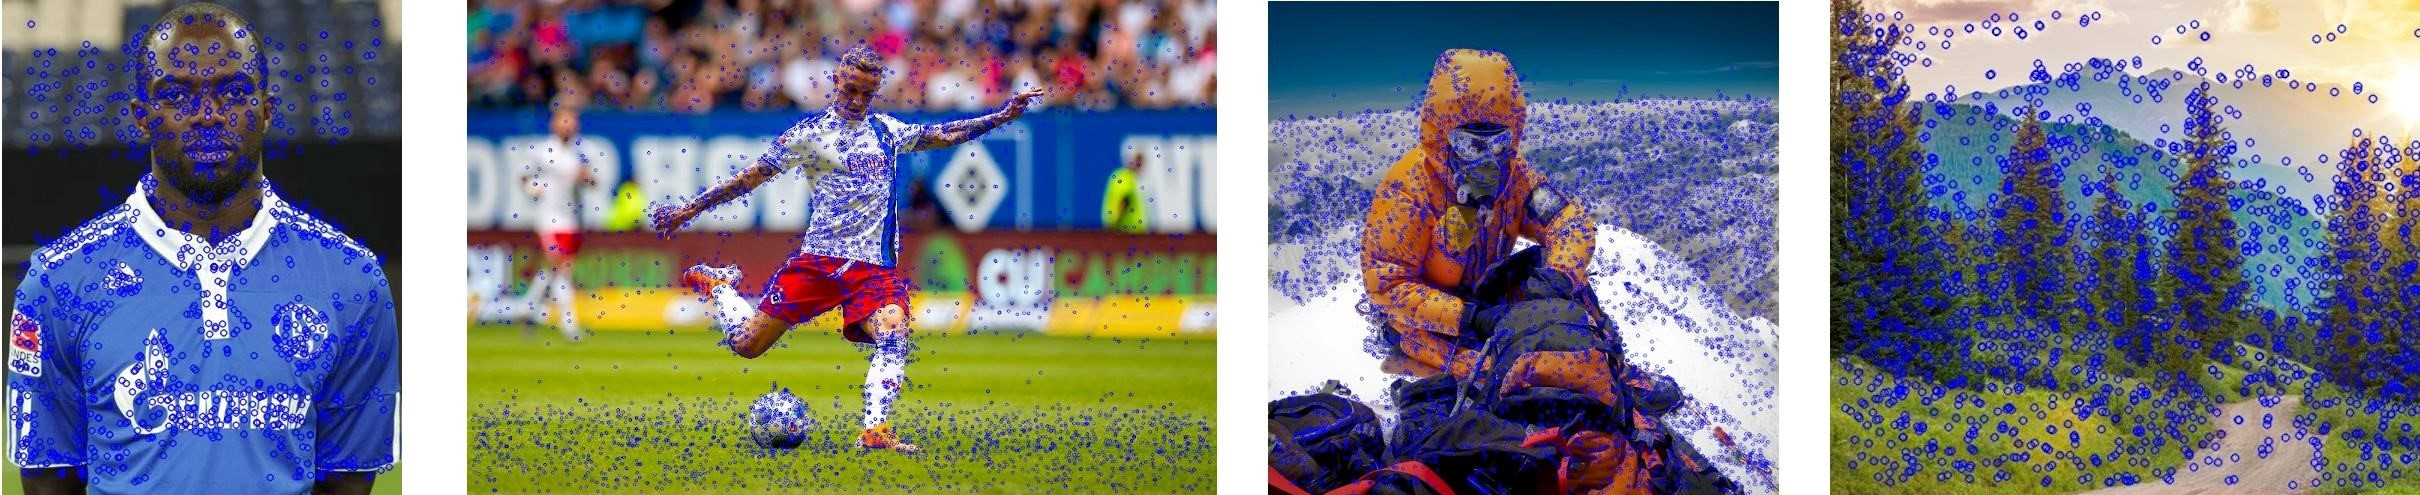
\includegraphics[scale=0.72]{keypoints.jpg}
\label{fig:keypoints}
\caption{Vier Beispielbilder mit blau markierten Keypoints ermittelt durch einen SURF-Detektor}
\end{center}
\end{figure}

\subsection{Keypoint Description}
Die Java-Klasse \textit{DescriptorExtractor} berechnet zu jedem Keypoint einen Feature-Vektor, welcher unterschiedliche Informationen enthält. Je nach Keypoint-Detektor, der vorher angewandt wurde, werden unterschiedich viele Eigenschaften ermittelt. Nach einer Reihe von Tests haben wir uns für den SURF-Detektor entschieden, da dieser bezüglich Rechengeschwindigkeit die anderen Detektoren deutlich überbietet. Der \textit{Speeded Up Robust Features} Algorithmus erzeugt dabei Features mit 64 Dimensionen. 

\subsection{Signaturen}
Da Bilder oftmals tausende von Keypoints beinhalten können, ist ein Vergleich aller Keypoints nicht zielführend. Deshalb wird im Bereich Computer Vision oft mit Signaturen oder Histogrammen gearbeitet. Da wir im späteren Verlauf Distanzen auf Basis der Earth Mover's Distance berechnen wollen, haben wir uns in einem frühen Stadium für den Einsatz von Signaturen entschieden. Beim Konzept der Signaturen werden ähnliche Keypoints geclustert und ihre Deskriptoren zu repräsentativen Feature-Vektoren zusammengefasst. Dabei kann jedes Bild unterschiedlich viele Signaturen mit einer unterschiedlichen Anzahl an Keypoints, sogenannten Gewichten, enthalten.
\\
\\
Beliebte Algorithmen zum Clustern von Features sind der k-Means-Algorithmus sowie DBSCAN (Density-Based Spatial Clustering of Applications with Noise). Beim k-Means-Verfahren wird für jedes Bild eine statische Anzahl an $k$ Clustern bestimmt. Da die Anzahl an Clustern in einem Bild Einfluss auf die Qualität der einzelnen Signaturen hat, haben wir uns für den DBSCAN-Algorithmus entschieden. Der DBSCAN-Algorithmus ist ein dichtebasierter Algorithmus, bei dem die Anzahl an Clustern dynamisch bestimmt wird. Dieser basiert auf der Annahme, dass zwei Objekte als \textit{dichte-verbunden} gelten, wenn es eine Kette von \textit{dichten} Objekten gibt, die diese Punkte miteinander verbinden. Die dadurch verbundenen Punkte bilden ein Cluster. Der Algorithmus verfügt über zwei Parameter $\epsilon$ und $minPts$. Dabei definiert $\epsilon$ die maximale Länge, bei der zwei Punkte als Nachbarn gelten, wenn die Distanz zwischen ihnen  $< \epsilon$ ist. Der Parameter $minPts$  bestimmt wann Objekte als \textit{dicht} gelten. Undzwar wenn es mindestens $minPts$ über $\epsilon$ erreichbare Nachbarn gibt.
\\
\\
Bei der Implementierung des DBSCAN-Algorithmus wurde die Klasse \textit{DBSCANClusterer} aus dem Package \textit{org.apache.commons.math3.stat.clustering} von Apache verwendet. Für die Signaturen wird der Mittelwert über jedes Feature der einzelnen Deskriptoren gebildet, welches in das entrpechende Cluster fallen. Dadurch ensteht im Fall von SURF ein zentrierten Feature-Vektor mit 64 Dimensionen der repräsentativ für das gesamte Cluster ist. Zusätzlich wird das Gewicht jeder Signatur abgespeichert, damit diese bei der Distanzberechnung miteinfließen können.

\subsection{Ähnlichkeitsmaß}
Auf Basis der zuvor ermittelten Signaturen werden im nächsten Schritt Distanzfunktionen eineführt um die Ähnlichkeit zwischen Objekten zu messen. Dabei werden die Earth Mover's Distnace und der Jaccard-Koeffizient zur Distanzberechnung näher betrachtet.
\\
\\
Als erstes haben wir einen Ansatz gewählt bei welchem wir die Distanzen aller Signaturen zueinander berechnen und mit den zuvor ermittelten Gewichten multiplizieren und dann durch das Gesamtgewicht teilen. Die Distanz zwischen zwei angenommen dreidimensionalen Signaturen würde sich somit wie folgt berechen: 
\\
\\
$d = dist * (24 + 7))/ (233 + 75) = 0,4026$,
\\
\\
wobei 
\\
\\
$dist = \left( \begin{array}{c} 3 \\ 6 \\ 9 \end{array}\right) - \left( \begin{array}{c} 2 \\ 4 \\ 8 \end{array}\right)$.
\\ 
\\
\\
Dabei hat Signatur $s_{1} = (3,6,9)^{T}$ ein Gewicht von $24$ und Signatur $s_{2} = (2,4,8)^{T}$ ein Gewicht von $7$. Das Bild von Signatur $s_{1}$ hat über alle Signaturen summiert ein Gewicht von 233 und das Bild von Signatur $s_{2}$ ein Gewicht von 75.
\\
\\
Diese Methode brachte uns jedoch unbefriedigende Ergebnisse, da eine solche Distanzfunktion keine wünschenswerten  Eigenschaften aufweist. Beispielsweise kann die Distanz zu einem identischen Bild nie Null sein, wenn mindestens ein Bild mehr als eine Signatur hat. Ebenso ist die Distanzfunktion auch nicht skalierungs- und rotationsinvariant. 
\\
\\ 
Eine etwas anspruchvollere Funktion ist die Earth Mover's Distance. Diese löst ein Optimierungsproblem und interpretiert dabei  die Signaturen des einen Bildes als Erdhaufen und die Signaturen des anderen Bildes als Erdlöcher. Ziel ist es dabei die gesamte Erdmasse von $A$ (Gesamtgewicht von Bild $A$) in die Löcher von $B$ (Gesamtgewicht von Bild $B$) zu befördern, wobei die zurückgelegte Gesamtdistanz zwischen $A$ und $B$ minimiert werden soll. Die Gesamtdistanz ergibt sich aus den Distanzen der einzelnen Signaturen von $A$ und $B$ multipliziert mit der Erdmasse (Gewicht von $A$), die auf diesen Strecken befördert wird. Für Löcher oder Erdhaufen, die aufgrund von unterschiedlichen Gesamtgewichten zweier Bilder übrig bleiben, wird ein Strafwert je Einheit zur Gesamtdistanz aufaddiert.
\\
\\
Auch für dieses Problem haben wir eine Klassenbibliothek in Java gefunden, die viele Funktionen der Earth Mover's Distance implementiert. Die JAR-Datei \textit{JFastEMD} beinhaltet unter Anderem eine \textit{Signature-}Klasse, an welche wir den zentrierten Feature-Vektor eines unserer Cluster sowie das entsprechende Gewicht übergeben. Das Interface \textit{Feature} definiert die Eigenschaften eines Features innerhalb einer Signatur, wobei es durch die Klasse \textit{Feature2D} implementiert wird. In \textit{Feature2D} wird mit zweidimensionalen Features gearbeitet sowie eine Methode zur Berechnung von euklidischen Distanzen mittels der Funktion \textit{groundDist(Feature f)} implementiert. Da wir in unserem Fall mit eindimensionalen Features arbeiten, welche im Vektor vom Typ \textit{double[]} vorliegen, mussten wir die JAR-Datei modifizieren und das Interface \textit{Feature} sowie die Klasse \textit{Feature2D} verändern. Die Klasse \textit{Feature2D} haben wir in \textit{Feature1D} umbennant, wobei wir dort zusätzlich neben der Funktion zur Berechnung der euklidischen Distanz eine Funktion zur Berechnung der Hamming-Distanz implementiert haben. Die Hauptklasse \textit{JFastEMD} berechnet dann schließlich die Earth Mover's Distance mit Hilfe der zuvor genannten Hilfsklassen. Die Methode zur Berechnung der Earth Mover's Distance sieht wie folgt aus:
\\
\\
$double$ $distance(Signature signature1, Signature signature2, double extraMassPenalty)$,
\\
\\
wobei der Paramter \textit{extraMassPenalty} den Strafwert für übrig gebliebene Erde definiert. Bei $-1$ wird je Einheit die höchste Distanz der beiden Signaturen zur Gesamtdistanz aufaddiert. Be $0$ ist der Strafwert $0$. Alle anderen positiven Werte ergeben fixe Strafwerte.
\\
\\
Hier etwas über Jaccard ... 

\subsection{Anfrageform und Indexierung}
Hier etwas über unseren Output im Folder outputImages sowie die Indexierung...

\subsection{Schlussfolgerung}
Hier etwas über unserer Schlussfolgerung über die Implementierung. Was man hätte anders machen können...


\section{Ergebnisse}
Test von verschiedenen Distanzfunktionen (Jaccard, EMD), verschiedern Penalty-Werte für EMD sowie Verwendung Distanzmaße (euklidisch, Hamming). Eventuell verschiedene Parameter bei DBSCAN-Clustering testen.

\subsection{Schlussfolgerung}

\FloatBarrier

\section{Ausblick}

\section{Arbeitsaufteilung}

\end{document}
